\documentclass[aspectratio=169]{beamer}
\usetheme{Madrid}
\usecolortheme{beaver}
\usepackage[utf8]{inputenc}
\usepackage[T1]{fontenc}
\usepackage{tikz}
\usepackage{amssymb}
\usepackage{graphicx}
\setbeamertemplate{navigation symbols}{}
\setbeamercolor{title}{fg=white,bg=cyan!60!black}
\setbeamercolor{frametitle}{fg=white,bg=cyan!50!black}
\setbeamercolor{block title}{bg=cyan!15,fg=black}
\setbeamercolor{block body}{bg=cyan!5,fg=black}

\title{G2 — Variables \& State}
\subtitle{Lesson 3: Health Bar}
\author{ByteForge --- Grade 7 --- Game Maker}
\date{}

\begin{document}

\begin{frame}
    \titlepage
\end{frame}

\begin{frame}{A variable driving TWO different things}
    \Large
    health drives a bar's WIDTH directly — the "one variable, automatically reflected in visuals" pattern behind every health/progress bar.

    \begin{center}
    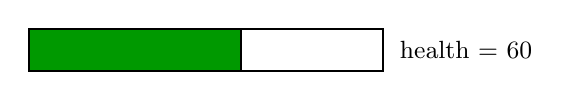
\begin{tikzpicture}[scale=0.9]

        \draw[thick] (0,0) rectangle (5,-0.6);
        \draw[thick, fill=green!60!black] (0,0) rectangle (3,-0.6);
        \node[right] at (5.1,-0.3) {\small health = 60};
    \end{tikzpicture}
    \end{center}
\end{frame}

\begin{frame}{A variable driving TWO different things --- Worked Example}
    \Large
    Worked example: health at 100 draws a full-width bar; health at 20 draws a bar only one-fifth as wide — the SAME width calculation (health / max * barWidth) every single frame, no special "low health" case needed.
\end{frame}

\begin{frame}{Your Turn}
    \Large
    Open the student map, find \textbf{G2 — Variables \& State}, and complete
    the \textbf{Health Bar} challenge --- everything you just saw, they now do themselves.
\end{frame}

\end{document}
